\chapter{Quadcopter Test}

\section{Introduction}

The main objective of this project is to determine the pose estimation accuracy of an airborne quadcopter in the outdoors, where the pose is a six-dimensional translation and angular orientation vector. This can be done by comparing a quadcopter's on-board pose estimate with the pose measurement of an external measurement tool. 

In Chapters meme and meme, a computer vision pose measurement system (CVS) was designed and tested and its pose measurement error was determined. It was found that the pose measurement data produced by the CVS is very complex, high dimensional and strongly inter-dimensionally dependant, as showed by the covariance matrix of Equation meme. This makes it hard to estimate the measurement error for any given pose measurement vector produced by the CVS.\@ 

Machine learning models are known to be able to detect underlying relationships in the data, if properly designed and trained. A radial basis function neural network (RBFNN) was trained to be able to do this, since they have been proven to work well with complex, noisy and non-linear data. The accuracy of the trained RBFNN was verified by an additional data set and is ready to be used in a real test. 

The trained RBFNN was used with data gathered from a test flight from a quadcopter. This chapter sets out to discuss the design and details of the tests performed, including the testing procedure, conditions and data processing. Then, the results are given and discussed, followed by a brief conclusionary discussion on the data and results gathered thus far. 

\section{Test Design and Procedure}

\subsection{Introduction}

\subsection{Test Design}

\subsubsection{Equipment}

The equipment required for the test are given as:

\begin{itemize}
    \item CVS camera and laptop.
    \item SunKopter quadcopter.
    \item Qualified model aeroplane pilot.
    \item Calibration board.
    \item 
\end{itemize}

The details of the CVS has been discussed before in Chapter meme. It consists of a camera, which captures the image data, and a laptop, which records and processes the data. A qualified pilot is required for safety reasons, since the quadcopter will be flown in close proximity to people and equipment. The calibration board is used in conjunction with the CVS to provide the pose data of the quadcopter. Here, the calibration board is an A3-sized\footnote{$297mm\times432mm$}, $6\times5$ square chessboard pattern calibration board. 

The SunKopter quadcopter is a custom-built quadcopter for the Solar and Thermal Energy Research Group's (STERG) research purposes. It is FISIESE SPECS EN MODEL NR EN VERWYS NA SPEC SHEET\@.

\subsubsection{Location}

The testing site where the flight tests were conducted is located at the Mariendahl experimental farm, owned and operated by Stellenbosch University (SU). It is also the location of STERG's Helio100 central receiver concentrated solar power (CSP) project. 

\subsubsection{Nog?}

\subsection{Test Procedure}

\subsubsection{Test Conditions and Layout}

The flight tests were conducted on the 26$^{th}$ of June, 2015 at the Helio100 test site at Mariendahl. The weather conditions were close to ideal with very little wind and clear skies. See Appendix MEME for a more detailed weather and wind report recorded on site.

For the test, video data of the SunKopter with a calibration board attached to its underside was recorded, where the pose data will be extracted offline afterwards. The issue of turbulence introduced by a quadcopter flying to close to the ground was considered, since it can negatively affect the flight performance of a quadcopter. A general rule of thumb to prevent ground effects from influencing flight, as stated by~\cite{basson-flight-test}, is to fly a quadcopter the length of one of its props from the ground. The CVS's camera was therefore placed on top of a 2m post, which eliminated ground effects from the flight tests.

A licensed back-up pilot was employed during the test. His responsibility was to perform the manual piloting tasks, such as positioning the SunKopter and switching modes as well as taking over the piloting of the SunKopter and safely land it in case the flight stability is compromised and a catastrophic failure is inevitable.

\subsubsection{Test Scenarios}

For each flight test, the SunKopter was manually positioned above the centre of the CVS's camera on the post and set to `loiter' mode. In this mode, the SunKopter will attempt to hold the altitude, position and yaw angle it had when it was set to loiter mode, while remaining stable, meaning that the SunKopter will attempt to hold a roll and pitch angle of $\ang{0}$. 

It has been established in Chapter meme that the pose measurement data from the CVS is highly inter-dimensionally dependant, which implies that the accuracy of the pose measurement will depend on the current pose relative to the CVS's camera. As a consequence of this, it was decided that several flight tests would be conducted, each with a slightly different distance or yaw angle relative to the CVS's camera. 

Distances of 1m and 2m from the camera were used. In preliminary testing it was found that distances greater than 2m from the camera, the CVS's starts losing view of the corners on the calibration board and struggles to detect and extract the corner coordinate data from the calibration board, making it impossible to perform the pose estimation. Furthermore, given that a quadcopter is symmetric about both of its axes, the yaw angles were set to $\ang{0}$, $\ang{22.5}$ and $\ang{45}$. 

Two sets of data was recorded during the flight test: one from the CVS and another from the onboard sensor suite of the quadcopter, which provides orientation and translation data. These two data sets will eventually allow the onboard pose estimation accuracy of the SunKopter to be determined. 

\subsubsection{Nog?}

\subsection{Data Processing}

\subsubsection{Introduction}

After the video data of the SunKopter with the calibration board attached was recorded, the data processing stage could begin. There are three different processing phases, which are the pose data extraction from the video data, data recentring around a common centre and finally determine the pose estimation accuracy of the SunKopter. Each of these phases are discussed in this section. 

\subsubsection{Pose Data Extraction}

The first step in the data processing phase is to extract the pose data of the calibration board, and by extension the SunKopter to which it was attached. This was done by using the process discussed in Chapter meme, where OpenCV's chessboard corner detector and PnP problem solver are used to extract six-dimensional pose information of a chessboard pattern calibration board. This process is fairly automated, however the output from the PnP solver required some conditioning.

The coordinate system for the corner detector and PnP solver used was specified in square units, i.e.\ a $5\times6$ square chessboard would have dimensions of $5\times6$ units. This required the translation vector to be transformed back to the SI unit by multiplying the PnP solver's output by 0.05, since each square on the chessboard is $5cm\times5cm$. The orientation vector is output in radians, which was converted to degrees. 

The CVS's camera captures video data at 30 frames per second, while the Pixhawk on the SunKopter sends data to the ground control station at a frequency of 20Hz, making it necessary to change the time scale of either data set. The Pixhawk's data packets contain various parameters, such as the battery voltage and altitude, but only the position and orientation data sets are of interest here. However, these data sets are not sent with every data package coming from the Pixhawk and do not necessarily arrive together either. It is therefore necessary to synchronise the position and orientation data sets from the Pixhawk.

To synchronise the data, a zero-order-hold was applied to each data set by using the timestamps for each data sample. What this means is that the value of each sample is held constant until it is updated by the next sample. Furthermore, the CVS's pose data was downsampled by selecting a sample from the set that coincides with the timestamps from the SunKopter's pose data set. 

\subsubsection{Data Centring}
\label{sec:chap5-data-centring}

After the pose data has been extracted from the video data, the CVS's pose estimate and the SunKopter's on-board pose estimate must be recentred to a common axis system. The CVS's axis system is centred around its camera centre, while the SunKopter's pose data is centred around the point where it is launched from. Therefore, to be able to compare the two sets of data, the constant offset vector between the axis systems must be determined. The axis systems and offset vector is demonstrated in Figure~\ref{fig:chap5-flight-test-schem}.

\begin{figure}
  \centering
  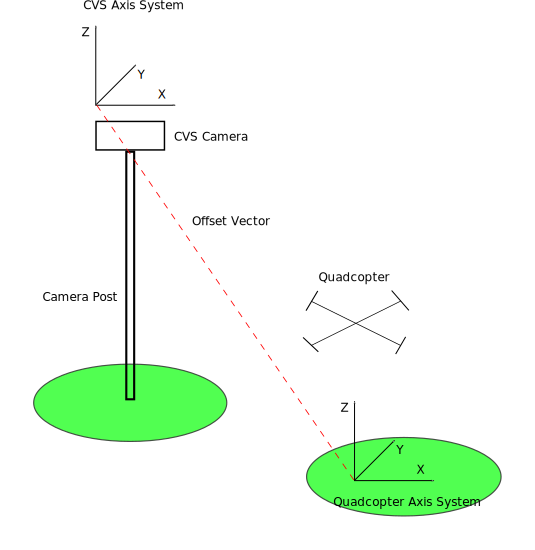
\includegraphics[width=0.8\textwidth]{figures/chapter5/test_flight_schem}
  \caption[Shematic of the test flight layout.]{Schematic of the test flight, the qaudcopter and CVS's respective axis systems and the offset vector between them.}
\label{fig:chap5-flight-test-schem}
\end{figure}

Furthermore, any angular offset for the CVS camera or the SunKopter, due to uneven ground conditions or camera placement, is also included in the offset vector. This makes the offset vector a six-dimensional translation and orientation pose vector. 

The offset vector is a constant value and is related to the quadcopter and CVS's pose estimate by the relation given in Equation~\ref{eq:chap5-pose-offset}, where $P$ is a six-dimensional pose vector. 

\begin{equation}
  \label{eq:chap5-pose-offset}
  P_{quadcopter} = P_{cvs} + P_{offset}
\end{equation}

In Equation~\ref{eq:chap5-pose-offset}, the $P_{offset}$ term is the unknown term. The pose data contained within the $P_{quadcopter}$ and $P_{cvs}$ terms contains noise in each sample, which requires that an optimisation procedure be used to find a offset vector that best relates the two sets of pose data. For the optimisation procedure, the error term in Equation~\ref{eq:chap5-err-func} was minimised, where the $e$ term is given by Equation~\ref{eq:chap5-err-term}. 

\begin{equation}
  \label{eq:chap5-err-func}
  \sqrt{\displaystyle\sum_{i=1}^{n} e_i^2}
\end{equation}

\begin{equation}
  \label{eq:chap5-err-term}
  e = P_{cvs} + P_{offset} - P_{quadcopter}
\end{equation}

The minimisation was done using the `minimize' function from the SciPy\footnote{SciPy v0.13.3} library and makes use of the \emph{BFGS} quasi-Newton method described by~\cite{nocedal2006numerical}. 

\subsubsection{Determining the Pose Estimation Error}

With the two data sets now directly relatable, the pose estimation error of a quadcopter in flight, the SunKopter in this case, can now be determined using the radial basis function neural network (RBFNN) discussed in Chapter meme. 

The input to the network is the CVS's pose data set. The network then outputs its error estimate for every sample, allowing a measurement error band to be drawn around the data. This band can then be used to determine if the quadcopter's pose estimate or the CVS's pose estimate is more accurate: when the quadcopter's estimate falls within the error band, it can be assumed that the quadcopter's pose estimate is more accurate for that sample then the CVS's is, while the opposite holds true if it falls outside the error band. It can then be determined which of the two systems produce, on average, the most accurate pose results. However, if it is found that the quadcopter's pose estimate is more accurate, one might be liable to ask if the CVS is still necessary.

Up to this point, any measure of the error in a quadcopter's pose estimation has been unavailable to outdoor quadcopters, except their on-board pose estimates which cannot be used to determine their own accuracy. This means that even if it is found that the quadcopter's pose estimate is more accurate than the CVS's, the CVS pose data will still provide a measure of the quadcopter's pose estimate which was not available previously. The outcome of this comparisson may lead to two outcomes.

If the quadcopter's pose estimate is more accurate than the CVS's, then the pose measurement error of the CVS can be taken as a worst-case measurement, where the quadcopter's pose estimate will always be at least as accurate as the CVS's. Conversely, if it is found that the CVS produces better pose measures, then the quadcopter's pose estimation error will be given by the difference between the CVS and quadcopter's pose data. 

\section{Results}

\subsection{Offset Vector}

Using the procedure described in Section~\ref{sec:chap5-data-centring}, the optimal offset vector relating the quadcopter and CVS's axis systems is given in Equation~\ref{eq:chap5-offset-result}. 

\begin{equation}
  \label{eq:chap5-offset-result}
  P_{offset} = 
  \begin{bmatrix}
    -6.61m & -0.834m & -4.17m & \ang{6.15} & \ang{62.7} & \ang{-185} \\
  \end{bmatrix}^T
\end{equation}

The translation values roughly coincide with the conditions that were recorded on site: the SunKopter was launched some distance from the CVS equipment for safety reasons. The launch site was slanted and located below the post on which the CVS's camera was placed. Thus, from a sanity standpoint, the offset that the optimisation procedure produced is a correct one. 

\subsection{Pose Estimation Error}

Fout histogramme + gem en std afwyking
Normale resultate
Test cloud

The pose estimation error was performed with the flight test data from the flight scenario where the SunKopter was flown 1$m$ from the CVS's camera and at a yaw angle of $\ang{0}$. 

Before the new flight test data was fed to the RBFNN, it was first checked that the test data falls within the training data limits. This is done to ensure that the RBFNN is not exposed to data for which its output will be inaccurate, which it will be if it was not trained to handle data in that range. Figure~\ref{fig:chap5-ts-tr-scatter} shows scatter plots for the test and training data dimensions and shows that the test data falls comfortably within the training data set. 

\begin{figure*}
  \centering
  \begin{subfigure}{0.9\textwidth}
    \includegraphics[clip, trim = 120 40 120 0, width=\textwidth]{figures/chapter5/ts_v_tr_pos}
    \caption{Position data.}
  \end{subfigure}
  ~
  \begin{subfigure}{0.9\textwidth}
    \includegraphics[clip, trim = 120 40 120 0, width=\textwidth]{figures/chapter5/ts_v_tr_orient}
    \caption{Orientation data.}
  \end{subfigure}
  \caption[Scatter plots of flight data vs. training data. ]{Scatter plots showing that the flight test data falls within the training limits. }
  \label{fig:chap5-ts-tr-scatter}
\end{figure*}

The results for the flight test are presented in Figure~\ref{fig:chap5-results}. Here, six figures are given which plot the six different pose dimensions. Each plot contains the SunKopter's pose estimate, as well as the measurement error margin for the CVS as was given by the RBFNN. 
  
\begin{figure*}
  \centering
  \begin{subfigure}{0.45\textwidth}
    \includegraphics[clip, trim = 150 0 120 0, width=\textwidth]{figures/chapter5/x}
    \caption{$x$}
  \end{subfigure}
  \begin{subfigure}{0.45\textwidth}
    \includegraphics[clip, trim = 150 0 120 0, width=\textwidth]{figures/chapter5/roll}
    \caption{Roll}
  \end{subfigure}
  \begin{subfigure}{0.45\textwidth}
    \includegraphics[clip, trim = 150 0 120 0, width=\textwidth]{figures/chapter5/y}
    \caption{$y$}
  \end{subfigure}
  \begin{subfigure}{0.45\textwidth}
    \includegraphics[clip, trim = 150 0 120 0, width=\textwidth]{figures/chapter5/pitch}
    \caption{Pitch}
  \end{subfigure}
  \begin{subfigure}{0.45\textwidth}
    \includegraphics[clip, trim = 150 0 120 0, width=\textwidth]{figures/chapter5/z}
    \caption{$z$}
  \end{subfigure}
  \begin{subfigure}{0.45\textwidth}
    \includegraphics[clip, trim = 150 0 120 0, width=\textwidth]{figures/chapter5/yaw}
    \caption{Yaw}
  \end{subfigure}
  \caption[Plots of the SunKopter's flight and measurement errors.]{Plots of the SunKopter's pose estimate with the error margins from of the CVS's pose measurement. }
  \label{fig:chap5-results}
\end{figure*}

The first important aspect to note of the plots in Figure~\ref{fig:chap5-results} is that the quadcopter's estimate largely falls within the error boundaries for the CVS's pose measurement, as given by the RBFNN. This means that the pose estimate given by the quadcopter's sensor suite is more accurate then the CVS's. The RBFNN has been adequately trained in Chapter meme and Figure~\ref{fig:chap5-ts-tr-scatter} shows that the test data falls within the training data limits, giving a degree of certainty that the quadcopter's true position falls within the extreme CVS pose measurement errors. It therefore follows that the measurement error of the CVS can be taken as a worst-case pose estimation error for the SunKopter. 

Second, there are sections in the CVS error estimate plots which are missing. The reason for this is that during the video recording, the CVS's camera lost its view of parts of the calibration pattern and OpenCV's pose estimator could therefore not extract the pose data for the calibration board for the frames where all of the corners were not visible. Furthermore, in some parts of the video, the pose estimator still sometime failed to extract pose data even when all of the corners were visible. This was somewhat remedied by adjusting the pose extractor to use an adaptive threshold filter on the video data and it is therefore suspected that poor and uneven lighting conditions during the test led to data not being extracted from some frames. 

\section{Conclusion}


